\documentclass[oneside,12pt]{book}
\usepackage[utf8]{inputenc}
\usepackage{standalone}
\usepackage[margin=2.5cm]{geometry}
\usepackage{graphicx}
\usepackage{hyperref}
\usepackage{lmodern}
\usepackage{float}
\usepackage[spanish]{babel}
\usepackage{csquotes}
\usepackage[figurename=Ilustración]{caption}
\usepackage[numbers]{natbib}
\usepackage{ragged2e}
\usepackage{array}
\usepackage{multirow}
\usepackage{parskip}
\usepackage{listings}
\usepackage{epigraph}
\usepackage{lipsum}

\usepackage{algorithm}
\usepackage{algpseudocode}

\usepackage{glossaries}

\makeglossaries

\newglossaryentry{latex}
{
    name=latex,
    description={Is a markup language specially suited for scientific documents}
}

\newglossaryentry{maths}
{
    name=mathematics,
    description={Mathematics is what mathematicians do}
}
% Glosario de términos - END

%\usepackage{fancyhdr}
\usepackage{geometry}
\usepackage{color}\usepackage{graphicx,xcolor}

\renewcommand{\lstlistingname}{Algoritmo}
%\renewcommand{\lstlistlistingnam%e}{Índice de~\lstlistingname s}

\floatname{algorithm}{Algoritmo}
\renewcommand{\listalgorithmname}{Índice de~\lstlistingname s}


\lstset{
        basicstyle=\fontsize{7}{11}\ttfamily,
        language=Java,
        captionpos=b,
}

\usepackage{titlesec}
\setcounter{secnumdepth}{3}
\titleformat{\chapter}[display]
{\normalfont\huge\bfseries}{\chaptertitlename\ \thechapter}{20pt}{\Huge}

\urlstyle{same}
\title{Diseño y desarrollo de un sistema empotrado basado en bus CAN con acceso inalámbrico para la monitorización de un vehículo automóvil}
\author{Gorka Eymard Santana Cabrera}
\date{Curso 2025 - 2026}
\renewcommand{\contentsname}{Contenido}
\renewcommand{\figurename}{Ilustración}
\usepackage{pifont}
\renewcommand\labelitemi{\ding{52}}

\begin{document}
%\maketittle
\input{Portada.tex}

%\newgeometry{margin=1.5cm}

\thispagestyle{empty}

%\lhead{ 
\begin{tabular}{p{15cm}p{5cm}}
  %
\includegraphics{Ilustraciones/LogoEII.jpg}   &  TFT04\\
  
\includegraphics[width=7cm]{Ilustraciones/NuevoLogoEII.png}   &  TFT04\\
\end{tabular}
%}

\vspace{1em}
\fboxrule=2pt
\begin{center}
\fcolorbox{gray}{gray!10}{\parbox{.8 \textwidth}{ {\large SOLICITUD DE DEFENSA DE TRABAJO DE FIN DE TÍTULO}}}
\end{center}

\vspace{1em}
\justify
D./Dª Gorka Eymard Santana Cabrera, autor del trabajo Diseño y desarrollo de un sistema empotrado basado en bus CAN con acceso inalámbrico para la monitorización de un vehículo automóvil, correspondiente a la titulación Grado de Ingeniería Informática.

\vspace{1em}
SOLICITA

\vspace{1em}
que se inicie el procedimiento de defensa del mismo, para lo que se adjunta la documentación requerida, haciendo constar que 

[ ] se autoriza / [ ] no se autoriza la grabación en audio de la exposición y turno de preguntas.

\vspace{1em}
Asimismo, con respecto al registro de la propiedad intelectual/industrial del TFT, declara que:

[ ] Se ha iniciado o hay intención de iniciarlo (defensa no pública).

[ ] No está previsto.

\vspace{1em}
Y para que así conste firma la presente. (fecha en firma electrónica)

\begin{center}
%En Las Palmas de Gran Canaria, a día de mes de año

\vspace{1em}
El/La estudiante

\vspace{3em}
Fdo.------------------------
\end{center}

\begin{center}
\fcolorbox{gray}{white!10}{\parbox{.9\textwidth}{
{\tiny A rellenar y firmar \textbf{obligatoriamente} por el/la/los/las tutores}

En relación con la presente solicitud, se informa:{\tiny (firmar donde corresponda)}

\vspace{1em}
\begin{center}
\begin{tabular}{|p{\dimexpr.45\linewidth}|p{\dimexpr.45\linewidth}|}
%\begin{tabular}{|l|r|}
    \hline
   & \\
  Positivamente {\tiny (en  caso  de  detección  de  copia, esta firma quedará invalidada)}  & Negativamente {\tiny (justificación en TFT05)} \\
   & \\
   & \\
   & \\
   & \\
   & \\
   & \\
  Fdo.------------------------ & Fdo.------------------------  \\
     & \\

    \hline
\end{tabular} 

\end{center}

\vspace{1em}

}
}

\vspace{1em}

%\cfoot{
DIRECTOR DE LA ESCUELA DE INGENIERÍA INFORMÁTICA
%}

\end{center}

\restoregeometry

\clearpage

\newpage
\pagenumbering{roman}
%{\Large{\textbf{Agradecimientos}}}
%\begin{flushleft}
La realización de este Trabajo de Fin de Título no habría sido posible sin el apoyo y la colaboración de diversas personas e instituciones a las que deseo expresar mi más sincero agradecimiento.

En primer lugar, quiero agradecer a los profesores Antonio C.\ Domínguez Brito y Jorge Cabrera Gámez, por su dedicación, orientación y apoyo durante el desarrollo de este trabajo. Su experiencia y los consejos recibidos han sido fundamentales para encauzar el desarrollo de este proyecto en la dirección correcta.

Asimismo, agradezco al profesor Jorge Cabrera Gámez, tutor colaborador, su implicación y el valioso apoyo técnico aportado durante las distintas fases del trabajo. Sus indicaciones han contribuido de manera significativa a la calidad del resultado final.

De igual modo, deseo expresar mi gratitud a la División de Robótica y Oceanografía Computacional del Instituto Universitario SIANI de la Universidad de Las Palmas de Gran Canaria, por poner a disposición de este proyecto los medios materiales y el equipamiento necesarios para llevar a cabo el desarrollo experimental y las pruebas del sistema.

Por último, agradezco a todas las personas que, de una forma u otra, han brindado su apoyo durante este período, haciendo posible la culminación de este trabajo.
\end{flushleft}


%\clearpage
{\setlength{\parskip}{8mm}
{\huge{\textbf{Resumen}}}

La estructura de este documento es orientativa. Las \textbf{partes obligatorias (motivación y objetivos, competencias, aportaciones, alineamiento ODS, desarrollo, conclusiones y bibliografía)} deben estar recogidas, aunque pueden reordenarse o redistribuirse en base a las características del trabajo.

    {EL presente Trabajo de Fin de Título(TFT) desarrolla un sistema empotrado basado en bus CAN que trabaja en la capa de aplicación de OBDII permitiendo la realización de diagnósis de vehículos. El sistema ha sido diseñado y validado tomando como referencia la arquitectura de comunicaciones de los vehículos del grupo VAG (Volkswagen Audi Group), cuya topología de \textit{Gateway} central es representativa de los vehículos modernos de la plataforma PQ25.}

\newpage

{\huge{\textbf{Abstract}}}


    {\large{Ahora en inglés:
    This Final Degree Project (TFT) develops an embedded system based on the CAN bus that operates at the OBD-II application layer, enabling vehicle diagnostics. The system has been designed and validated against the communication architecture of Volkswagen Audi Group (VAG) vehicles, whose central \textit{Gateway} topology is representative of modern PQ25 platform vehicles.
 }

}}
\tableofcontents

%\addcontentsline{toc}{section}{Listings}
%\lstlistoflistings
%\listofalgorithms 

\listoffigures

\listoftables


\clearpage
\pagenumbering{arabic}

\chapter{Introducción}
\section{Introducción a la Comunicación en el Sector Automovilístico}

La evolución del sector automovilístico durante las últimas décadas se ha caracterizado
 por una transición acelerada de sistemas puramente mecánicos a arquitecturas altamente
 electronificadas. Los vehículos modernos no son solo máquinas de combustión o motores
 eléctricos, sino complejas redes de computadoras sobre ruedas que albergan decenas de 
 Unidades de Control Electrónico (ECU). Estas ECU gestionan todo, desde la inyección de
combustible y los frenos ABS hasta el infoentretenimiento. Para que esta arquitectura distribuida funcione, es imperativo un sistema de comunicación robusto y en tiempo real. Es aquí donde surge el bus CAN (Controller Area Network). Desarrollado originalmente por la empresa Bosch en 1986 y estandarizado a nivel global en 1993 bajo la norma ISO 11898, el bus CAN nació para resolver el problema del cableado excesivo, permitiendo que múltiples microcontroladores y dispositivos se comuniquen entre sí sin depender de una computadora central, garantizando alta tolerancia al ruido electromagnético y priorización de mensajes críticos.\\

\begin{figure}[!bp]
\centering
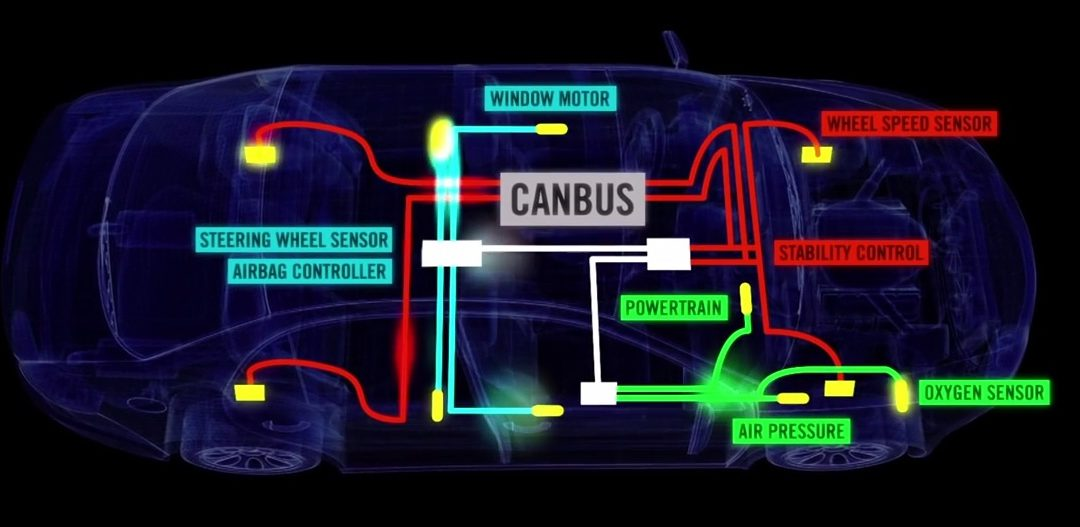
\includegraphics[width=0.5\textwidth]{Ilustraciones/CAN_Car.jpg}
\caption{Imagen ilustrativa de un bus CAN en un vehículo, mostrando la interconexión entre varias ECU a través de un par de cables trenzados. Fuente: \url{https://serviciosdelautomovilarca.es/2021/02/07/sistema-can-bus-en-el-automovil/}.}
\label{fig:CAN_CAR}
\end{figure}


A nivel técnico, el bus CAN es un protocolo de comunicaciones en serie de tipo diferencial, lo que significa que utiliza dos cables (CAN High y CAN Low) para transmitir la información, logrando una excelente inmunidad frente a interferencias electromagnéticas. Funciona bajo un paradigma multimaestro y utiliza un mecanismo de resolución de colisiones no destructivo basado en la prioridad del mensaje (CSMA/CD+AMP). En lugar de enviar información a direcciones específicas, el bus CAN transmite tramas o frames a toda la red. Cada trama contiene un identificador único; cuanto menor es el valor numérico de este identificador, mayor es la prioridad del mensaje en el bus. Esto asegura que la información crítica, como los comandos de frenado, tenga siempre preferencia sobre datos secundarios.\\

\begin{table}[!htbp]
\caption{Estructura de una Trama CAN Estándar 2.0A.}
\label{tab:trama_can}
\centering
\begin{tabular}{|l|c|p{9cm}|}
\hline
\textbf{Campo} & \textbf{Bits} & \textbf{Descripción (Funcionamiento Básico)} \\ \hline
\textbf{SOF} & 1 & \textit{Start of Frame}: Indica el inicio de la transmisión. \\ \hline
\textbf{Identificador (ID)} & 11 & Define la prioridad y el contenido del mensaje. \\ \hline
\textbf{RTR} & 1 & \textit{Remote Transmission Request}: Diferencia entre trama de datos o petición. \\ \hline
\textbf{Control} & 6 & Indica la longitud de los datos que le siguen. \\ \hline
\textbf{Datos} & 0 - 64 & La carga útil (hasta 8 bytes de información, p.ej., valor de RPM). \\ \hline
\textbf{CRC / ACK / EOF} & Varios & Comprobación de errores, confirmación de recepción y fin de trama. \\ \hline
\end{tabular}%
\end{table}

Aunque el bus CAN define cómo viajan los bits por los cables (las capas física y de enlace de datos del modelo OSI), no especifica el "idioma" de los datos en sí. Para que equipos de diagnóstico externos puedan interpretar universalmente la información del vehículo (como las RPM, la temperatura del refrigerante o los códigos de error), la industria adoptó protocolos estandarizados de la capa de aplicación. El más fundamental es el OBD-II (On-Board Diagnostics), obligatorio en Estados Unidos desde 1996 y en Europa (como EOBD) desde principios de los 2000. OBD-II define un conector físico estándar de 16 pines (SAE J1962) y un conjunto de identificadores de parámetros (PID) que cualquier herramienta puede solicitar. Con la llegada de los vehículos modernos, el estándar ISO 15765-4 dictaminó cómo deben encapsularse y enviarse estos mensajes OBD-II a través del bus CAN físico. Además, para diagnósticos más profundos a nivel de fabricante, la industria utiliza actualmente el estándar UDS (Unified Diagnostic Services, ISO 14229), que permite operaciones avanzadas como la lectura de variables propietarias o el flasheo de centralitas.



\section{Introducción a los Protocolos de Comunicación}

El sistema desarrollado en este TFT se apoya en una pila de protocolos estándar 
ampliamente adoptada en el sector de la automoción. Cada capa cumple una función 
específica y bien delimitada, desde la transmisión física de bits hasta la 
interpretación de los datos de diagnosis a nivel de aplicación.


\subsection{CAN Bus \textemdash\ ISO 11898}

El \textit{Controller Area Network} (CAN) es un bus serie multi-maestro desarrollado 
por Robert Bosch GmbH en 1983~\cite{Bosch91-can} y estandarizado bajo la norma 
ISO 11898~\cite{ISO11898-1-15}. Fue diseñado para permitir la comunicación entre 
múltiples unidades de control electrónico (ECUs) a través de un único par de cables 
trenzados, eliminando la necesidad de cableado punto a punto entre 
nodos~\cite{Bosch91-can}. Su mecanismo de arbitraje no destructivo basado en la 
prioridad del identificador de mensaje garantiza que no se produzcan colisiones en el 
bus, mientras que su señalización diferencial lo hace robusto frente al ruido 
electromagnético propio del entorno vehicular~\cite{ISO11898-1-15}. En este proyecto 
se utiliza CAN 2.0A con identificadores de 11 bits a una velocidad de 500 kbps, que 
es la velocidad estándar definida para el acceso OBD-II~\cite{SAE-J1979-12}.


\subsection{ISO-TP \textemdash\ ISO 15765-2}

El \textit{ISO Transport Protocol} (ISO-TP), definido en la norma 
ISO 15765-2~\cite{ISO15765-2-16}, es el protocolo de transporte utilizado sobre CAN 
en el contexto del diagnóstico vehicular. Su función principal es superar la 
limitación fundamental del bus CAN, cuyas tramas admiten un máximo de 8 bytes de 
\textit{payload}~\cite{ISO11898-1-15}: ISO-TP permite segmentar y reensamblar 
mensajes de hasta 4095 bytes mediante cuatro tipos de trama --- \textit{Single Frame} 
(SF), \textit{First Frame} (FF), \textit{Consecutive Frame} (CF) y \textit{Flow 
Control} (FC) ---, que gestionan el flujo de datos entre el escáner y la 
ECU~\cite{ISO15765-2-16}. En este proyecto, ISO-TP actúa como capa de transporte 
imprescindible para transmitir respuestas que exceden los 8 bytes, como el número de 
identificación del vehículo (VIN) o listas de códigos de avería (DTCs), y su 
implementación se apoya en la librería 
\texttt{python-can-isotp}~\cite{Menager23-isotp}.


\subsection{OBD-II \textemdash\ SAE J1979 / ISO 15031-5}

El estándar OBD-II (\textit{On-Board Diagnostics}, segunda generación), definido por 
la SAE J1979~\cite{SAE-J1979-12} y su equivalente europeo ISO 15031-5, establece una 
interfaz de diagnóstico normalizada que cualquier herramienta de escáner puede 
utilizar para interrogar a las ECUs de un vehículo. Sobre CAN, los mensajes OBD-II se 
transportan como \textit{payloads} ISO-TP~\cite{ISO15765-2-16}: el escáner envía una 
petición compuesta por un byte de modo y un byte de PID, y la ECU responde con los 
datos solicitados precedidos por el modo incrementado en 
\texttt{0x40}~\cite{SAE-J1979-12}. El estándar define varios servicios o modos, de 
los cuales este proyecto implementa cuatro: el Modo \texttt{0x01} para la lectura de 
datos en vivo (18 PIDs), el Modo \texttt{0x03} para la lectura de DTCs almacenados, 
el Modo \texttt{0x04} para el borrado de DTCs y el Modo \texttt{0x09} para la 
obtención del VIN del vehículo~\cite{SAE-J1979-12}.


\subsection{UDS NRC \textemdash\ ISO 14229-1}

El estándar UDS (\textit{Unified Diagnostic Services}), definido por la norma 
ISO 14229-1~\cite{ISO14229-1-20}, establece los servicios de diagnóstico de alto 
nivel utilizados en la comunicación entre herramientas de diagnosis y ECUs modernas. 
En el contexto de este proyecto, el elemento relevante de UDS son los 
\textit{Negative Response Codes} (NRC): cuando una ECU no puede atender una 
petición, responde con una trama de respuesta negativa con el formato 
\texttt{[0x7F, modo, código\_NRC]}, donde el código identifica la razón del 
rechazo~\cite{ISO14229-1-20}. Se implementan seis NRCs, entre ellos \texttt{0x11} 
(servicio no soportado), \texttt{0x12} (PID no soportado), \texttt{0x22} 
(condiciones incorrectas, por ejemplo intentar borrar DTCs con el motor en marcha) y 
\texttt{0x33} (acceso denegado por seguridad)~\cite{ISO14229-1-20}, dotando al 
simulador de un comportamiento fiel al de una ECU real.

\chapter{Estado actual y objetivos iniciales}
%\section{Motivación y antecedentes}

La motivación para el desarrollo de este trabajo surge de la curiosidad por estudiar la serie de protocolos que se usan en el sector automovilistico donde se trabaja en un entorno de comunicaciónes críticas y ruidosas, donde se requiere una alta fidelidad en la transmisión de datos.\\

\section{Objetivos}

El objetivo del desarrollo de este proyecto, es diseñar y desarrollar un sistema empotrado basado en bus CAN con acceso inalámbrico para la monitorización de un vehículo automóvil perteneciente al grupo de automoción VAG. Con el fin de tener una herramienta de monitorización y evaluación de los parámetros del vehiculo, que permita el acceso a los datos de forma inalámbrica, y que pueda ser utilizada para la mejora del rendimiento del vehículo, la detección de fallos y el mantenimiento predictivo.

Este es un CAPÍTULO \textbf{OBLIGATORIO}.
\section{Motivación y antecedentes}

La motivación para el desarrollo de este trabajo surge de la curiosidad por estudiar la serie de protocolos que se usan en el sector automovilistico donde se trabaja en un entorno de comunicaciónes críticas y ruidosas, donde se requiere una alta fidelidad en la transmisión de datos.\\

\section{Objetivos}

El objetivo del desarrollo de este proyecto, es diseñar y desarrollar un sistema empotrado basado en bus CAN con acceso inalámbrico para la monitorización de un vehículo automóvil perteneciente al grupo de automoción VAG. Con el fin de tener una herramienta de monitorización y evaluación de los parámetros del vehiculo, que permita el acceso a los datos de forma inalámbrica, y que pueda ser utilizada para la mejora del rendimiento del vehículo, la detección de fallos y el mantenimiento predictivo.

\chapter{Aportaciones del trabajo}
\chaptermark{Competencias, aportaciones y ODS}
%\section{Principales aportaciones}

Justificar qué es lo que este TFT \textbf{aporta} a nuestro entorno socio-económico, técnico o científico. Repercusión esperada.

\section{Competencias específicas}

Indicar, sólo para las \textbf{competencias específicas} relacionadas de forma más directa con el trabajo desarrollado, cómo se han cubierto con este TFT.

\section{Relación con los Objetivos de Desarrollo Sostenible (ODS)}

\begin{center}

\begin{table}[!htbp]
\caption{Grado de relación del TFT con los objetivos de desarrollo sostenible.}
\label{tab:ODS}
\centering
\begin{tabular}{|l|c|c|c|c|}
\cline{1-5}
  & \multicolumn{4}{c|}{Grado de relación} \\ \cline{2-5}
 ODS & 0 & 1 & 2 & 3 \\
  & No procede & Bajo & Medio & Alto \\
  \cline{1-5}
1 Fin de la Pobreza & X & & & \\ \cline{1-5}
2 Hambre cero & X & & & \\ \cline{1-5}
3 Salud y Bienestar & & X & & \\ \cline{1-5}
4 Educación de calidad & & & X & \\ \cline{1-5}
5 Igualdad de género & X & & & \\ \cline{1-5}
6 Agua limpia y saneamiento & X & & & \\ \cline{1-5}
7 Energía Asequible y no contaminante & & & X & \\ \cline{1-5}
8 Trabajo decente y crecimiento económico & & X & & \\ \cline{1-5}
9 Industria, Innovación e Infraestructuras & & & X & \\ \cline{1-5}
10 Reducción de las desigualdades & X & & & \\ \cline{1-5}
11 Ciudades y comunidades sostenibles & & X & & \\ \cline{1-5}
12 Producción y consumo sostenibles & & & X & \\ \cline{1-5}
13 Acción por el clima & & & X & \\ \cline{1-5}
14 Vida submarina & X & & & \\ \cline{1-5}
15 Vida de ecosistemas terrestres & X & & & \\ \cline{1-5}
16 Paz, justicia e instituciones sólidas & X & & & \\ \cline{1-5}
17 Alianzas para lograr objetivos & X & & & \\ \cline{1-5}
\end{tabular}%
\end{table}
\end{center}
\textbf{Justificar el grado de relación del TFT con cada uno de los ODS, indicando qué aspectos del trabajo contribuyen a cada uno de ellos.}
\\
ODS 9 (Medio - 3): Desarrollo de tecnología e innovación pura para el sector del mantenimiento industrial/automoción.\\
ODS 12 (Medio - 2): Fomenta el "Derecho a Reparar". Una buena diagnosis alarga la vida del coche y evita la chatarra tecnológica.\\
ODS 7 y 13 (Medio - 2): OBD-II vigila las emisiones de gases. Leer y arreglar los fallos de motor reduce la huella de carbono.\\
ODS 4 (Medio - 2): Proyecto muy didáctico, aplicable para que otros alumnos aprendan sobre CAN y bajo nivel.\\
ODS 3, 8 y 11 (Bajo - 1): Impacto indirecto. Ciudades menos contaminadas y apoyo al trabajo técnico de los talleres.

Este es un CAPÍTULO \textbf{OBLIGATORIO}.

También pueden incluirse parte de estos contenidos en las conclusiones, en la descripción de los objetivos o en forma de anexos.

\section{Principales aportaciones}

Justificar qué es lo que este TFT \textbf{aporta} a nuestro entorno socio-económico, técnico o científico. Repercusión esperada.

\section{Competencias específicas}

Indicar, sólo para las \textbf{competencias específicas} relacionadas de forma más directa con el trabajo desarrollado, cómo se han cubierto con este TFT.

\section{Relación con los Objetivos de Desarrollo Sostenible (ODS)}

\begin{center}

\begin{table}[!htbp]
\caption{Grado de relación del TFT con los objetivos de desarrollo sostenible.}
\label{tab:ODS}
\centering
\begin{tabular}{|l|c|c|c|c|}
\cline{1-5}
  & \multicolumn{4}{c|}{Grado de relación} \\ \cline{2-5} 
 ODS & 0 & 1 & 2 & 3 \\
  & No procede & Bajo & Medio & Alto \\  
  \cline{1-5} 
1 Fin de la Pobreza & X & & & \\ \cline{1-5}
2 Hambre cero & X & & & \\ \cline{1-5}
3 Salud y Bienestar & & X & & \\ \cline{1-5}
4 Educación de calidad & & & X & \\ \cline{1-5}
5 Igualdad de género & X & & & \\ \cline{1-5}
6 Agua limpia y saneamiento & X & & & \\ \cline{1-5}
7 Energía Asequible y no contaminante & & & X & \\ \cline{1-5}
8 Trabajo decente y crecimiento económico & & X & & \\ \cline{1-5}
9 Industria, Innovación e Infraestructuras & & & X & \\ \cline{1-5}
10 Reducción de las desigualdades & X & & & \\ \cline{1-5}
11 Ciudades y comunidades sostenibles & & X & & \\ \cline{1-5}
12 Producción y consumo sostenibles & & & X & \\ \cline{1-5} 
13 Acción por el clima & & & X & \\ \cline{1-5}
14 Vida submarina & X & & & \\ \cline{1-5}
15 Vida de ecosistemas terrestres & X & & & \\ \cline{1-5}
16 Paz, justicia e instituciones sólidas & X & & & \\ \cline{1-5}
17 Alianzas para lograr objetivos & X & & & \\ \cline{1-5}
\end{tabular}%
\end{table}
\end{center}
\textbf{Justificar el grado de relación del TFT con cada uno de los ODS, indicando qué aspectos del trabajo contribuyen a cada uno de ellos.}
\\% JUSTIFICACIONES ODS (IDEAS PARA REDACTAR):
ODS 9 (Medio - 3): Desarrollo de tecnología e innovación pura para el sector del mantenimiento industrial/automoción.\\
ODS 12 (Medio - 2): Fomenta el "Derecho a Reparar". Una buena diagnosis alarga la vida del coche y evita la chatarra tecnológica.\\
ODS 7 y 13 (Medio - 2): OBD-II vigila las emisiones de gases. Leer y arreglar los fallos de motor reduce la huella de carbono.\\
ODS 4 (Medio - 2): Proyecto muy didáctico, aplicable para que otros alumnos aprendan sobre CAN y bajo nivel.\\
ODS 3, 8 y 11 (Bajo - 1): Impacto indirecto. Ciudades menos contaminadas y apoyo al trabajo técnico de los talleres.

\chapter{Desarrollo}
%\section{Metodología}

Para el desarrollo del trabajo se ha seguido la metodología de desarrollo de software en cascada, que se compone de las siguientes fases: análisis, diseño, implementación y validación.

\section{Fases de desarrollo}

\subsection{Análisis}

En esta primera fase se han identificado los requisitos del sistema y se han estudiado los protocolos de comunicación empleados en los vehículos del grupo VAG (Volkswagen Audi Group) sobre la plataforma PQ25, para poder empezar con el diseño de la infraestructura de monitorización y comunicación con las distintas ECUs del vehículo.

Durante este análisis se ha descubierto que los vehículos del grupo VAG sobre la plataforma PQ25 utilizan una topología de \textbf{Gateway Central} esto lo que consigue es diferenciar los buses CAN de forma que no haya saturación de los datos en un solo CAN Bus. Esta arquitectura implica además que el bus CAN-Powertrain \textbf{no es directamente accesible desde el conector OBD-II}: el Gateway actúa como intermediario, filtrando y enrutando los mensajes entre buses, lo que impide el acceso directo al bus de motor mediante un adaptador CAN estándar conectado al puerto de diagnóstico. Podemos diferenciar entre:
\begin{itemize}
    \item \textbf{CAN-Powertrain}: este bus conecta la ECU (Motor), sensor ABS/ESP y transmisión. Este es el CAN Bus más importante con lo que tiene una velocidad de 500 kbps.
    \item \textbf{CAN-Diagnostic}: este es el bus de diagnositco que se revela en el puerto OBD-II situado en la parte inferior del salpicadero bajo el volante. Este es un bus que opera a 500 kbps.
    \item \textbf{CAN-Comfort}: este bus al no ser de alta prioridad tiene una velocidad de 100 kbps y controla elevalunas, cierre centralizado, iluminación interna, etc.
    \item \textbf{CAN-Infotainment}: este bus es el que controla los sistema de entretenimiento e información como la radio, navegación y bluetooth. Este bus también opera a 100 kbps.
\end{itemize}

En cuanto a la capa de Enlace y Red se encontró que se trabaja siguiendo las normas ISO(Organización Internacional de Normalización):
\begin{itemize}
    \item \textbf{ISO 11898-1}: este norma define el estándar físico y de enlace de datos del CAN Bus.
    \item \textbf{ISO 15765(CAN-TP)}: el protocolo de transporte. El CAN Bus estándar solo envía 8 bytes por mensaje, pero la ECU necesita de un protocolo de transporte que le permita enviar mensajes de más de 8 bytes para poder enviar por ejemplo, el VIN del vehículo(17 bytes), este protocolo le permite fragmentar los mensajes en varios mensajes de 8 bytes y luego reensamblarlos en el destino.
\end{itemize}

\subsection{Diseño}

Para el diseño del projecto se

Ajuste a la planificación inicialmente prevista.

Modificación en los objetivos planteados.

Este es un CAPÍTULO \textbf{OBLIGATORIO}.

\section{Metodología}

Para el desarrollo del trabajo se ha seguido la metodología de desarrollo de software en cascada, que se compone de las siguientes fases: análisis, diseño, implementación y validación.
\section{Fases de desarrollo}

\subsection{Análisis}

En esta primera fase se han identificado los requisitos del sistema y se han estudiado los protocolos de comunicación empleados en los vehículos del grupo VAG (Volkswagen Audi Group) sobre la plataforma PQ25, para poder empezar con el diseño de la infraestructura de monitorización y comunicación con las distintas ECUs del vehículo.

Durante este análisis se ha descubierto que los vehículos del grupo VAG sobre la plataforma PQ25 utilizan una topología de \textbf{Gateway Central} esto lo que consigue es diferenciar los buses CAN de forma que no haya saturación de los datos en un solo CAN Bus. Esta arquitectura implica además que el bus CAN-Powertrain \textbf{no es directamente accesible desde el conector OBD-II}: el Gateway actúa como intermediario, filtrando y enrutando los mensajes entre buses, lo que impide el acceso directo al bus de motor mediante un adaptador CAN estándar conectado al puerto de diagnóstico. Podemos diferenciar entre:
\begin{itemize}
    \item \textbf{CAN-Powertrain}: este bus conecta la ECU (Motor), sensor ABS/ESP y transmisión. Este es el CAN Bus más importante con lo que tiene una velocidad de 500 kbps.
    \item \textbf{CAN-Diagnostic}: este es el bus de diagnositco que se revela en el puerto OBD-II situado en la parte inferior del salpicadero bajo el volante. Este es un bus que opera a 500 kbps.
    \item \textbf{CAN-Comfort}: este bus al no ser de alta prioridad tiene una velocidad de 100 kbps y controla elevalunas, cierre centralizado, iluminación interna, etc.
    \item \textbf{CAN-Infotainment}: este bus es el que controla los sistema de entretenimiento e información como la radio, navegación y bluetooth. Este bus también opera a 100 kbps.
\end{itemize}

En cuanto a la capa de Enlace y Red se encontró que se trabaja siguiendo las normas ISO(Organización Internacional de Normalización):
\begin{itemize}
    \item \textbf{ISO 11898-1}: este norma define el estándar físico y de enlace de datos del CAN Bus.
    \item \textbf{ISO 15765(CAN-TP)}: el protocolo de transporte. El CAN Bus estándar solo envía 8 bytes por mensaje, pero la ECU necesita de un protocolo de transporte que le permita enviar mensajes de más de 8 bytes para poder enviar por ejemplo, el VIN del vehículo(17 bytes), este protocolo le permite fragmentar los mensajes en varios mensajes de 8 bytes y luego reensamblarlos en el destino.
\end{itemize}

\subsection{Diseño}

Para el diseño del projecto se 

Ajuste a la planificación inicialmente prevista.

Modificación en los objetivos planteados.

\chapter{Resultados}
%Presentación de los resultados del trabajo. Repercusión.


Presentación de los resultados del trabajo. Repercusión.

\chapter{Conclusiones y trabajo futuro}
%\section{Conclusiones}

Valoración de resultados, grado de consecución de los  objetivos.

\section{Trabajo futuro}

Líneas de trabajo futuro, aspectos pendientes, posibles extensiones.

\section{Uso de la IA}

Indicar el uso que se ha hecho de la IA tanto en la elaboración de este documento como en el desarrollo del TFG.

\vspace{1cm}

\textbf{EXTENSIÓN DE LA MEMORIA:}

\begin{itemize}
    \item GII, GIFM, DGII-ADE (parte de GII): entre 50 y 100 páginas
    \item GCID: entre 75 y 100 páginas
\end{itemize}

Este es un CAPÍTULO \textbf{OBLIGATORIO}.

\section{Conclusiones}

Valoración de resultados, grado de consecución de los  objetivos.

\section{Trabajo futuro}

Líneas de trabajo futuro, aspectos pendientes, posibles extensiones.

\section{Uso de la IA}

Indicar el uso que se ha hecho de la IA tanto en la elaboración de este documento como en el desarrollo del TFG.

\vspace{1cm}

\textbf{EXTENSIÓN DE LA MEMORIA:}

\begin{itemize}
    \item GII, GIFM, DGII-ADE (parte de GII): entre 50 y 100 páginas
    \item GCID: entre 75 y 100 páginas
\end{itemize}

\chapter{Otros capítulos y anexos}

El documento debe terminar con las \textbf{referencias bibliográficas} (SECCIÓN \textbf{OBLIGATORIA}). Después pueden incluirse \textbf{anexos} de forma opcional.

\section{Ejemplos de capítulos opcionales}

Dependiendo del tipo de trabajo, se podrían incluir, en el orden que corresponda, capítulos adicionales como los siguientes:

\begin{description}
\item{REQUISITOS}
\item{NORMATIVA Y LEGISLACIÓN} incluir la legislación vigente que afecte al TFT (ley de protección de datos, leyes sobre seguridad, ...)
\item{ASPECTOS ECONÓMICOS Y TEMPORALES}
\item{DISEÑO}
\item{RESULTADOS EXPERIMENTALES}
\item{MANUAL  DE  USUARIO  Y  SOFTWARE}  deberán  incluirse  obligatoriamente  en  la  memoria  los extractos más relevantes   del código desarrollado. Siempre que sea posible, deberá   proporcionarse acceso a un repositorio software.
\end{description}


\clearpage

\begin{thebibliography}{9}

\bibitem{Bosch91-can}
Robert Bosch GmbH,
\textit{CAN Specification Version 2.0},
Robert Bosch GmbH, Stuttgart, 1991.

\bibitem{ISO11898-1-15}
International Organization for Standardization,
\textit{ISO 11898-1:2015 -- Road vehicles -- Controller area network (CAN) --
Part 1: Data link layer and physical signalling},
ISO, Ginebra, 2015.

\bibitem{ISO15765-2-16}
International Organization for Standardization,
\textit{ISO 15765-2:2016 -- Road vehicles -- Diagnostic communication over
Controller Area Network (DoCAN) -- Part 2: Transport protocol and
network layer services},
ISO, Ginebra, 2016.

\bibitem{SAE-J1979-12}
Society of Automotive Engineers,
\textit{SAE J1979:2012 -- E/E Diagnostic Test Modes},
SAE International, Warrendale, 2012.

\bibitem{ISO14229-1-20}
International Organization for Standardization,
\textit{ISO 14229-1:2020 -- Road vehicles -- Unified diagnostic services (UDS) --
Part 1: Application layer},
ISO, Ginebra, 2020.

\bibitem{Menager23-isotp}
S. Ménager \textit{et al.},
\textit{python-can-isotp Documentation},
2023. Disponible en: \url{https://can-isotp.readthedocs.io/}

\bibitem{Twiss23-pythoncan}
python-can contributors,
\textit{python-can Documentation},
2023. Disponible en: \url{https://python-can.readthedocs.io/}

\end{thebibliography}

\printglossaries

\end{document}